\documentclass[letterpaper, 12pt]{article}
\usepackage{xcolor}
\usepackage{graphicx}
\usepackage{amsmath}
\usepackage{amsthm}
\usepackage{amssymb}
\usepackage{physics}
\usepackage{mathtools}
\usepackage{multicol}
\usepackage{tikz}
\title{Balance Integrator}
\author{Kevin Zheng}
\begin{document}
\maketitle
\begin{abstract}
	\par A description of a balance/scale that can integrate using torque.
	The left side is a point mass at 1 meter away, and the right side is a bent rod.
	The mass of the point mass should be the answer to the definite integral, while the right side should be of uniform mass. Notice that the way that the rod is bent is not necessarily the curve of the function we are trying to integrate.
\end{abstract}
\tableofcontents
\section{A prototype using varying density}
\par The left side is a point mass 1 meter away from the center, thus the torque from it is $\tau = mgr = mg$.
The right side is a straight bar, but with varying density.
\begin{center}
	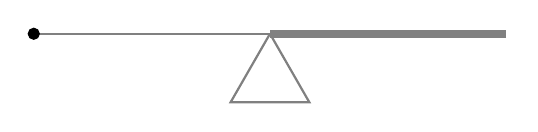
\begin{tikzpicture}
		\draw[gray, thick] (-3, 0) -- (0, 0);
		\filldraw[black] (-3, 0) circle (2pt);
		\draw[gray, thick] (0, 0) -- (1/2, -0.87) -- (-1/2, -0.87) -- (0, 0);
		\draw[gray, line width=1mm] (3, 0) -- (0, 0);
	\end{tikzpicture}
\end{center}
\begin{proof}
	Let $L$ be the length of the bar, $f(x)$ the function we wish to integrate, and $\rho(x)$ the density of the rod.
	\begin{align*}
		\tau &= \int_0^L xdF\\
		\tau &= \int_0^L xgdm\\
		\tau &= \int_0^L xg\rho(x)dx\\
	\end{align*}
	We want $\tau$ on the right side to be the same (in the opposite direction) as the $\tau$ on the left side.
	\begin{align*}
		mg &= \int_0^L xg\rho(x)dx\\
		mg &= g\int_0^L x\rho(x)dx\\
		m &= \int_0^L x\rho(x)dx\\
	\end{align*}
	And the mass should be the same value as our arbitrary integral ($\int_0^Lf(x)dx$).
	\begin{align*}
		\int_0^Lf(x)dx = \int_0^L x\rho(x)dx\\
	\end{align*}
	Although it is not true that the integral being the same implies the integrand is the same, the integrand being the same is \emph{a} solution and we will use it.
	\begin{align*}
		f(x) = x\rho(x)\\
		\rho(x) = \frac{f(x)}{x}
	\end{align*}
	This implies that manufacturing a rod with varying density $\rho(x)$ will have the same torque as a point mass with mass $\int_0^L f(x) dx$.
\end{proof}
\section{To address the problems of a rod with varying density}
We will attempt to investigate the possibility of achieving the same effect using a bent rod of uniform density instead of a straight rod of nonuniform density.
A varying density in the rod will have two drawbacks, the first being the difficulty of manufacturing one, and the second being the difficulty of visualizing the integrator at work.
\begin{center}
	\begin{tikzpicture}
		\draw[gray, thick] (-3, 0) -- (0, 0);
		\filldraw[black] (-3, 0) circle (2pt);
		\draw[gray, thick] (0, 0) -- (1/2, -0.87) -- (-1/2, -0.87) -- (0, 0);
		\draw[scale=1,domain=0:3,smooth,variable=\x,black]  plot ({\x},{\x * \x * (sin(\x*50) + 1)/10});
	\end{tikzpicture}
\end{center}
\begin{proof}
	Let $h(x)$ be the height of the bar with respect to the level of the scale.
	\begin{align*}
		\tau &= \int_0^L \sqrt{x^2 + h^2(x)}\times dF\\
		\tau &= \int_0^L \sqrt{x^2 + h^2(x)}\sin\theta dF\\
		% Add more figures here to better explain where \sin\theta comes from
		\tau &= \int_0^L \sqrt{x^2 + h^2(x)}\frac{x}{h(x)} dF\\
		\tau &= \int_0^L x\frac{\sqrt{x^2 + h^2(x)}}{\sqrt{h^2(x)}}dF\\
		\tau &= \int_0^L x\sqrt{\frac{x^2 + h^2(x)}{h^2(x)}}dF\\
		\tau &= \int_0^L x\sqrt{1 + \frac{x^2}{h^2(x)}}dF\\
		\tau &= \int_0^L x\sqrt{1 + \frac{x^2}{h^2(x)}}gdm\\
		\tau &= \int_0^L x\sqrt{1 + \frac{x^2}{h^2(x)}}g\rho dx\\
	\end{align*}
	In this case, $\rho$ is a constant, so we can take it out of the integral.
	If you so choose, you may simply assume that $\rho$ is 1.
	\begin{align*}
		\tau &= g\rho\int_0^L x\sqrt{1 + \frac{x^2}{h^2(x)}}dx\\
	\end{align*}
	Just like last time, we want $\tau$ on the right to be equal (in the opposite direction) to the $\tau$ from the point mass on the left.
	\begin{align*}
		m &= \rho\int_0^L x\sqrt{1 + \frac{x^2}{h^2(x)}}dx\\
	\end{align*}
	Also like last time, we want $m$ to be the answer to the integral $\int_0^L f(x) dx$
	\begin{align*}
		\int_0^Lf(x)dx &= \rho\int_0^L x\sqrt{1 + \frac{x^2}{h^2(x)}}dx\\
	\end{align*}
	Therefore, the integrands being the same is a solution to the above equation.
	\begin{align*}
		f(x) &= \rho x\sqrt{1 + \frac{x^2}{h^2(x)}}\\
		\frac{f(x)}{x\rho} &= \sqrt{1 + \frac{x^2}{h^2(x)}}\\
		(\frac{f(x)}{x\rho})^2 &= 1 + \frac{x^2}{h^2(x)}\\
		\frac{x^2}{h^2(x)} &= (\frac{f(x)}{x\rho})^2 - 1\\
		\frac{h^2(x)}{x^2} &= \frac{1}{(\frac{f(x)}{x\rho})^2 - 1}\\
		h^2(x) &= \frac{x^2}{(\frac{f(x)}{x\rho})^2 - 1}\\
		h(x) &= \sqrt{\frac{x^2}{(\frac{f(x)}{x\rho})^2 - 1}}\\
		h(x) &= \sqrt{\frac{x^4}{(\frac{f(x)}{\rho})^2 - x^2}}\\
		h(x) &= x^2\sqrt{\frac{1}{(\frac{f(x)}{\rho})^2 - x^2}}\\
	\end{align*}
\end{proof}
\end{document}
